\chapter{Struktura a vrstvy ovladačů}
  Zde si popíšeme jednotlivé vrstvy ovladačů a jejich vzájemnou návaznost, pro
  doplnění uvedeme obrázek, který celou situaci znázorňuje graficky.
  \section{Prostor jádra}
  Jak jsme si výše uvedli, karty \com\ a \comx\ jsou založené na odlišných
  typech součástek, je
  tedy nutné mít pro tyto dva druhy karet dva ovladače. Ty stojí v~nejnižší
  vrstvě softwarového vybavení a mají jména \emph{cesplx} a \emph{cespcr}.
  Umožňují zápis do paměťových prostorů karty, obsluhují a předávají přerušení
  vyšším vrstvám, \emph{cesplx} navíc provádí \dma\ přenosy, dále uveďme
  například čtení konfigurací a další operace s~hardware. \\ \indent
  Nad tímto jádrem dalších ovladačů leží sjednocující ovladač se
  jménem \emph{combo6}. Ten,
  kromě nezávislosti na spodní vrstvě, také zaštiťuje operace nad
  speciálním souborem\footnote{v~UN*Xových systémech slouží speciální soubory
  ke komunikaci ovladače a programu v~uživatelském prostoru. Implementovanými
  operacemi (otevření, zápis, čtení, \ldots) se ale nikterak neliší od
  obyčejného souboru, mohou být tedy použita stejná systémová
  volání.}. \\ \indent
  Nad tímto nezávislým celkem nelze než očekávat opět závislé
  ovladače, tentokrát ale konkrétních designů. Ke každému designu existuje
  samostatný ovladač, který si s~výstupem ať už jeho, nebo zpracovaným výstupem
  \ppc\ programu, poradí. \\ \indent
  Je třeba zmínit jednu výjimku, \emph{Scampi} a \nflow\ ovladače
  používají ještě další \emph{scampi} vrstvu nad \emph{combo6}
  ovladačem (tedy souběžně s~designovým),
  která předává pakety z~designového ovladače do uživatelského prostoru, jak
  se čtenář dozví dále.
  \section{Uživatelský prostor}
  Pro jednotlivé designy existují nástroje, které vědí jak spolupracovat
  s~jadernými moduly a jak se chovat k~výstupu z~nich. Pomocí výše zmíněného
  speciálního souboru a obyčejných síťových rozhraní začne nástroj komunikovat
  a zpracovávat data v~uživatelském prostoru. V~některých případech není nutné
  mít žádný nástroj, design se v~kooperaci s~ovladači chová jako obyčejná
  síťová karta.
  \begin{figure}[h]
    \begin{center}
      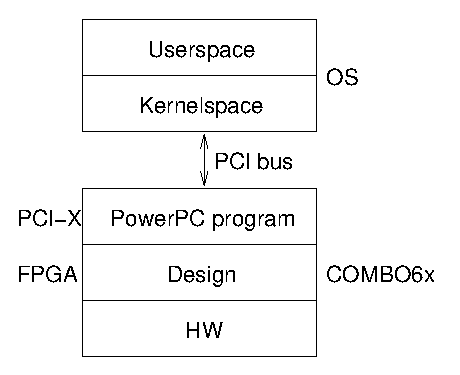
\includegraphics[height=5cm]{layers}
      \caption{Vrstvy znázorněné obrázkem}
    \end{center}
  \end{figure}

\chapter{Cesta k~ovladačům}
  Jako první meta byl stanoven přepis starších ovladačů umístěných přímo
  v~jádře do formy modulů. Následovala implementace ovladače pro novější typ
  karty, \comx, odladění funkčnosti včetně \dma\ přenosů a testování pomocí
  rozvíjejícího se projektu \emph{FlowMon}, kterým podle zadání práce máme
  ověřit správnou funkčnost, což zahrnuje i naprogramování samotného ovladače
  pro tento design, jak si ověříme později.
  \section{LKM}
  \subsection{Implementace}
  Na počátku bylo třeba prostudovat samotné rozhraní a objasnit systém
  přidávání ovladačů za běhu.
  Systém ke konfiguraci systému používá \emph{autoconf}, nástroj
  využívající tabulek vygenerovaných při překladu samotného jádra (jsou
  uloženy v~jeho binárním srdci), po detekci jednotlivých kusů hardware,
  porovná tyto tabulky a
  zjistí, který ovladač má tuto konkrétní oblast na starosti. Zkusí zavolat
  jeho vlastní funkci a pokud odpoví kladně (ano, tuto komponentu umím
  ovládat), předá mu řízení a pokračuje dále. Tento děj se odehrává při
  spuštění systému a pokud systém nepodporuje modulární binární kód (tuto
  možnost můžeme při konfiguraci jádra zakázat), už jej nikdy
  neopakuje\footnote{nesmíme opomenout uvažovat tzv, \uv{horká} zařízení,
  vezměme například \emph{USB},
  kde tuto proceduru po samotném připojení do jisté míry jádro také
  provádí, avšak pro zjednodušení můžeme uvážit statický systém}. \\ \indent
  V~opačném případě může být vyvolán i později, a proto je nutné ovladač
  trochu přihnout. Jednak je
  potřeba tabulky dynamicky doplnit a jednak je potřeba oznámit systému změnu
  tabulek, aby provedl znovu detekci karet a ostatních komponent podle nového
  nastavení. Dobře zdokumentované \emph{API}\footnote{Application Program
  Interface,
  aplikační rozhraní programu} nám poskytne několik maker\footnote{funkce,
  jejíž tělo překladač nahradí za jeho všechna volání ještě před překladem;
  často
  používaná metoda v~jazyce C}, jak docílit vytvoření správných prototypů
  řádek zmíněných tabulek, následně dokumentace odkáže na volání funkcí, jak
  tyto řádky do tabulky zařadit a přepis je kompletní. \\ \indent
  Logicky provedeme stejnou transformaci u všech dosavadních ovla\-da\-čů až na
  pojmenování řádků závisejících na jméně modulu. K~oproštění se od zbytečné
  redundance stejného kódu přišly opět ke slovu makra jazyka C, s~jejichž
  pomocí se text popsaný v~předchozích odstavcích objevuje v~projektu jen
  jednou a je před překladem automaticky rozmnožen do každého modulu zvlášť,
  ovšem s~jiným obsahem. \\ \indent
  Změna poté spočívá pouze ve vytvoření adresářů pro jednotlivé moduly,
  rozkopírovaní stávajících souborů do těchto nových adresářů a přidání
  zdrojového souboru do každého tohoto adresáře s~následujícím obsahem:
\begin{verbatim}
#include <cesmod.h>

static int loc[] = { -1, -1 };
static const char * const cespcr_attrs[] =
                        { "combobridge", NULL };
CESNET_MODULE(cespcr, cespcr_attrs, "pci", "pci", pci);
\end{verbatim}
  Prvním řádkem vložíme definici CESNET\_MODULE makra (jeho obsah je možné
  vidět na přiloženém CD, nebo přímo v~CVS), poté nastavíme
  lokátory (parametry) pro rodičovské zařízení, v~tomto případě \emph{pci}
  sběrnici,
  jak vidíme v~3. a 4. parametru makra. Druhý parametr jsou atributy --
  jméno předávané potomkům, v~našem případě modulu \emph{combo6}.
  Zbývá poslední parametr, ten se v~makru spojí s~koncovkou \emph{\_names} a
  tato externí proměnná \emph{pci\_names} obsahuje jména lokátorů, tedy těch
  dvou $-1$, které nastavujeme jako \emph{loc}. \\ \indent
  Během této práce narážíme na problém s~modulem \emph{combo6} (později i
  \emph{scampi}). Tyto ovladače narozdíl od ostatních implementují operace nad
  speciálním souborem, jejich moduly musíme definovat jiným způsobem, pomocí
  MOD\_DEV a nikoliv MOD\_DRV,
  jak jej máme použito v~našem vytvořeném makru. Uvědomme si, že definice
  pomocí MOD\_DRV za nás obstará vřazení záznamu do tabulek a znovu-projití
  hardware a srovnání s~prvky tabulky. Tento nedostatek vyřešíme vložením
  obsahu makra do souborů pro tyto dva moduly a adekvátní úpravou spočívající
  ve volání oněch funkcí. Definice proměnných poté vypadá takto:
\begin{verbatim}
static const char * const combosix_attrs[] =
                { "combobus", NULL };
CFDRIVER_DECL(combosix, DV_DULL, combosix_attrs);
extern struct cfattach combosix_ca;
extern const struct cdevsw combosix_cdevsw;

extern const char *nullcf_locnames[];
static int loc[] = { };
static struct cfparent combosix_par[] = {
        { "combobridge", "cesplx", DVUNIT_ANY },
        { "combobridge", "cespcr", DVUNIT_ANY }
};
static struct cfdata combosix_cf[] = {
        { "combosix", "combosix", 0, FSTATE_STAR,
                loc, 0, &combosix_par[0],
                nullcf_locnames },
        { "combosix", "combosix", 0, FSTATE_STAR,
                loc, 0, &combosix_par[1],
                nullcf_locnames },
};
\end{verbatim}
  a kód v~inicializačním bloku (bez ošetření chybových cest, ty jsme zde pro
  jednoduchost vynechali):
\begin{verbatim}
config_cfdriver_attach(&combosix_cd);
config_cfattach_attach(combosix_cd.cd_name,
                &combosix_ca);
config_cfdata_attach(&combosix_cf[0], 1);
config_cfdata_attach(&combosix_cf[1], 1);
\end{verbatim}
  Funkce pro deinicializaci se nese v~podobném duchu -- s~výjimkou
  obráceného pořadí volání funkcí a změnou \emph{attach} na
  \emph{detach}. \\ \indent
  Spolu s~tímto přechodem se s~minimálními úpravami daří vytvoření a spuštění
  binárního kódu na \nbsd\ verze 3.0 a nic nám nebrání vytvoření ovladačů pro
  samotnou kartu \comx.
  \subsection{Operace s~LKM}
  Každý operační systém podporující modulární kód obsahuje nějaký způsob,
  jak moduly do jádra vložit. U \nbsd\ je to skupina uživatelských
  programů, jejichž název má na počátku \emph{mod}. Vložení ovladače obstarává
  \emph{modload}, v~příkazovém řádku následovaný jménem souboru s~modulem
  včetně koncovky
  \emph{.o} (objekt). Tímto byl modul přidán do jádra, to automaticky zavolalo
  jeho inicializační funkce a začíná pracovat. \\ \indent
  Ke zjištění jmen modulů pracujících v~jádře lze spustit \emph{modstat} a po
  zjištění jména můžeme opačným postupem k~přidávání, modul odebrat. To
  zařídí poslední z~trojice příkazů \emph{modunload} následovaný jménem
  modulu, tentokrát již bez přípony. Tyto aspekty fungování je třeba zanést do
  dokumentace probírané v~příštích kapitolách, jelikož i to je cíl naší práce.
  \section{Tvorba COMBO6x NIC ovladače}
  Výchozí bod pro nás v~tomto okamžiku je \nic\ ovladač pro \com.
  Protože hradlové pole spolu s~designy doznalo změn, jenž nejsou kompatibilní
  se staršími díly, vymažeme z~něj úseky odpovídající za přerušení, příjem a
  vysílání paketů, pozměníme inicializační část a zůstane nám tak pouze
  bazální kostra. Ve schopnostech ovladače tedy chybí obsluha a
  uskutečnění \dma\ přenosů, korektní obsluha přerušení a jiné potřebné věci,
  které nebylo možné implementovat před ustálením vývoje
  firmware a usměrněním metod vývoje programů do instrukční paměti \ppc\
  procesoru karty. \\ \indent
  Nezávislá mezivrstva \emph{combo6} zůstane zachována, rozšíříme ji pouze o
  pár nových možností, které nebudou starší spodní vrstvou a ovladači designů
  využívané.
  \section{NetBSD rozhraní}
  K~tomu, abychom mohli vytvořit ovladač, korektně obsluhovat přerušení,
  \dma\ přenosy a další, musíme prostudovat manuálové stránky s~rozhraním
  systému a poté naše znalostí využít ve smyslu následujících odstavců.
  \subsection{Obsluha přerušení}
  Při této události, která může přerušit a odložit vykonávání aktuálně
  zpracovávaného kódu, musíme v~prvním kroku zjistit, zda jej opravdu vyvolala
  naše karta. \emph{IRQ} může být sdílené více ovladači, jelikož počet
  ovladačů a
  obsluhovaného hardware může převyšovat počet možných přerušení (na novějších
  architekturách mají výrobci procesorů snahu tento počet zvýšit). Ověření
  provedeme přečtením stavového registru karty, který bude nastaven právě když
  karta vyvolala přerušení. \\ \indent
  Pokud jsme přesvědčeni o pravosti přerušení, obsloužíme jej dále
  v~závislosti na vyvolané události. Může to být několik typů, jednak jej může
  z~nějakého důvodu vyvolat \ppc\ program, jednak samotný design, čili \fpga\ a
  konečně může oznámit dokončení \dma\ přenosu (také z~\ppc\
  programu). V~každém z~těchto tří případů pouze předáme s~vhodným parametrem
  přerušení vyšším, designovým vrstvám, které jej dále obslouží podle jejich
  vlastního uvážení, zavolání přerušení je závislé na použitém \fpga\ designu
  a k~němu odpovídajícímu \ppc\ programu. \\ \indent
  \nbsd\ k~tomuto účelu používá stejný způsob, jako ostatní operační systémy.
  Při inicializaci ovladače zaregistrujeme obsluhovací funkce, která je pak
  automaticky při přerušení zavolána. Při odebrání ovladače zmíněnou funkci
  odregistrujeme podobným způsobem.
  \subsection{DMA}
  Po upřesnění předchozích pojmů můžeme přistoupit k~jedné z~hlavních
  oblastí, jimiž se má práce rozsáhleji zabývat. Máme navrhnout, vytvořit a
  zdokumentovat programové vybavení pro přenosy v~módu \emph{Bus Master DMA}
  mezi \emph{PCI}
  kartou \comx\ a paměťovým systémem hostitelského počítače. Pusťme se tedy do
  práce. Jako první si určíme směr a tendenci implementace. Nejprve je třeba
  inicializovat proměnné a nachystat prostor v~paměti, nad kterým budeme
  operace přenosů provádět. Je třeba si uvědomit, že karta (a ostatní zařízení)
  nemají obecně schopnost adresovat celý paměťový prostor architektury,
  a proto je nutné
  využít funkce operačního systému, aby byl zajištěn takový prostor, kam
  konkrétní hardware přistupovat může. \\ \indent
  V~\nbsd\ jsou pro tento případ k~dispozici funkce se jmény začínající na
  \emph{bus\_dmamap\_}. Abychom se
  později o alokaci a mapování paměti ve většině případů nemuseli starat,
  provedeme tyto operace při nahrávání ovladače, v~\emph{attach} funkci.
  Poté budeme připravený prostor používat po celou dobu, kdy bude ovladač
  v~paměti a nakonec zavoláme funkce s~opačným efektem v~reverzním pořadí,
  tentokrát ve funkci \emph{detach}, volané při odebírání ovladače. \\ \indent
  Jak velký prostor potřebujeme a jaké bude jeho uspořádání? Jednak lze pomocí
  \dma\ přenosů z~karty číst její konfiguraci, připravíme tedy blok o velikosti
  konfigurační struktury následovaný malou oblastí s~ukazatelem na tato data
  jak v~adresním prostoru hostitelském, tak karty. Jednak si připravíme celý
  blok struktur obsahující pozice v~pamětech hostitele a karty pro každý možný
  přenosový zásobník zvlášť (pro design \nic\ je jich pro příjem a výdej po 256,
  dohromady tedy 512). Pro přijímací struktury ještě vytvoříme prostory pro
  příjem dat o velikosti 1536 oktetů\footnote{8 bitů, tento pojem se používá
  v~souvislosti se síťovými technologiemi} a ukazatele rovnou do těchto
  struktur přiřadíme. Pro vysílání takto
  budeme činit až dynamicky, při požadavku od jádra na odeslání paketu.
  Tyto vytvořené oblasti pro příjem určují místa, do kterých má \ppc\
  program nahrát zpracovaná data, popř. odkud si je
  může vyvolat, v~závislosti na směru přenosu. Struktury, do nichž tyto
  ukazatele přiřazujeme, jsou podobné té
  za konfigurační oblastí, obsahují ale pouze tři údaje -- adresu na kartě,
  stav a délku přenosu.
  \subsection{Režim komunikace}
  V~předchozí podkapitole můžeme zaregistrovat náznak popisu komunikace,
  uveďme ji tedy na pravou míru. V~podstatě máme dva směry komunikace.
  Jeden směr, příjem paketů, přichází zezdola,
  naopak odesílání seshora ve smyslu uspořádání hardware--uživatelský prostor
  (hardware je pochopitelně spodní vrstva v~tomto uspořádání).
  \subsubsection{Příjem paketů}
  Data se po průchodu několika vrstvami dostanou až do \ppc\ programu.
  V~tomto okamžiku program naplní stavový ukazatel počtem přijatých bajtů,
  struktury v~\dma\ oblasti (připomeňme, že tato oblast je nastavena od vložení
  ovladače do jádra) naplní aktuálními daty a konečně, změní stav přerušení,
  čímž jej vyvolá. Ovladač zjistí příčinu (příchod dat),
  zruší stav přerušení a provede čekání na dokončení \dma\ přenosu. V~tuto
  chvíli má k~dispozici data a v~další fázi postačuje přeposlat pakety
  konkrétnímu síťovému rozhraní, jehož identifikátor lze mimo jiné přečíst ze
  stavového registru. Tím máme hotovu první část.
  \subsubsection{Odesílání paketů}
  \ppc\ program umí
  operovat se dvěma frontami, pokud je jedna aktivní, budeme plnit do druhé a
  naopak. Je tedy nutné uchovávat ukazatel na frontu, jenž byla použita dříve
  (není právě aktivní) a ten použijeme k~identifikaci fronty, do které data
  zapíšeme. \\ \indent
  Z~uživatelského prostoru dojde k~zápisu do rozhraní, jádro nám ulehčí práci
  a překopíruje paket do struktury v~oblasti jádra a zavolá naší funkci
  obstarávající vysílání
  a my zde můžeme obsah a délku paketu a identifikaci rozhraní vložit do
  fronty k~odesílání a odstartovat přenos. \\ \indent
  \ppc\ program zjistí změnu, start přenosu, začne jej tedy provádět, opět
  si za pomoci \dma\ přenese potřebná data a pošle je do designu. Po ukončení
  opět vyvolá přerušení, aby uvědomil ovladač o dokončení a ten mohl uvolnit
  paměť vytvořenou před samotným přenosem.
  \subsection{Implementace}
  Jelikož již máme všechny potřebné znalosti, provedeme nyní podle zmíněné
  komunikace implementaci. \\ \indent
  Naši práci začneme příjmem paketů, to je jednodušší, protože se nemusíme
  starat
  o dvě fronty. Do obsluhy přerušení, které nám předá nejspodnější vrstva naší
  hierarchie (\emph{cespcr}), přidáme následující řádky:
\begin{verbatim}
if (xmask & PCRDMA_INTR_RX_MASK)
        cge_recv(sc);
if (xmask & PCRDMA_INTR_ERR_MASK)
        printf("combo6 pcidma error IRQ!\n");
\end{verbatim}
  Proměnnou \emph{xmask} nám předá nižší vrstva, je to přečtený stavový
  registr přerušení (\emph{PCR\_INTR\_STAT}), který mění \ppc\ program. Je
  v~něm uloženo, k~jaké události došlo, my jej zde otestujeme a pokud se
  jedná o příchod paketu (\emph{PCRDMA\_INTR\_RX\_MASK}), zavoláme naší funkci
  pro příjem. Druhá možnost, chybové přerušení, značí, že je něco v~přenosech
  v~nepořádku, upozorníme tedy uživatele výpisem zprávy. Sám \ppc\ program
  na kartě
  obstará přerušení vykonávání další práce tím, že zastaví přenosy, od této
  chvíle tedy nebude vyvoláno žádné další přerušení. \\ \indent
  Podívejme se nyní podrobněji na \emph{cge\_recv}. Její jediný parametr
  funkce je \emph{sc}, soukromá struktura ovladače, máme v~ní uloženy všechny
  potřebné informace včetně ukazatele na poslední použitou strukturu z~bloků,
  jak jsme si vysvětlili výše. Celá implementace této funkce spočívá v~jednom
  cyklu probíhajícím stále dokola, dokud není stav programem
  změněn na dokončeno --
  v~tomto úseku to byl poslední paket (\emph{DMA\_FLAGS\_DONE\_MASK}). Poté
  cyklus skončí a my jsme s~prací hotovi. \\ \indent
  V~těle cyklu jako první zjistíme, kde jsme skončili v~minulém přenosu podle
  zmíněného ukazatele a zde budeme i pokračovat tak, že přeneseme pomocí
  \dma\ stav a délku příchozího paketu. Samotný paket poté přeneseme v~plné
  délce přeneseme (opět pomocí \dma) a
  předáme jádru na další zpracování (\emph{ifp->if\_input}, kde ifp je
  rozhraní, kterému paket náleží). To automaticky uvolní tento zásobník,
  poslední prací tedy je vytvořit nové místo pro další paket, až opět
  dosáhneme stejné hodnoty v~ukazateli. \\ \indent
  Vysílání je postupem podobné, zvláštní je ale implementací dvou front. Po
  přijetí paketu od jádra (\emph{IFQ\_DEQUEUE(\&ifp->if\_snd, m)}, \emph{ifp}
  je opět rozhraní, \emph{m} je paket k~odeslání) do našeho ovladače, přidáme
  data z~tohoto paketu do jedné z~front pro vysílání (rozhodneme podle
  \emph{tx\_run} proměnné z~\emph{sc} struktury) přiřazením do \emph{x\_dmap}
  a odstartujeme samotný
  přenos. Ukončení přenosu nám karta oznámí přerušením, změníme tedy obsluhu
  následovně:
\begin{verbatim}
if (xmask & PCRDMA_INTR_RX_MASK)
        cge_recv(sc);
if (xmask & PCRDMA_INTR_TX_MASK)
        cge_send(sc);
if (xmask & PCRDMA_INTR_ERR_MASK)
        printf("combo6 pcidma error IRQ!\n");
\end{verbatim}
  Došlo-li k~ukončení přenosů, uvolníme paměť všech paketů a namapovanou oblast
  k~\dma\ přenosu:
\begin{verbatim}
if (sd->x_mbuf) { /* byl opravdu paket vlozen? */
        bus_dmamap_unload(sc->sc_dmat, sd->x_dmap);
        m_freem(sd->x_mbuf);
}
\end{verbatim}
  Opět tyto příkazy provádíme v~cyklu, pro každou jednotku vloženou do
  fronty. Tím jsme dokončili i vysílací část. Celou strukturu operací
  vidíme v~tomto diagramu:
  \begin{figure}[h]
    \begin{center}
      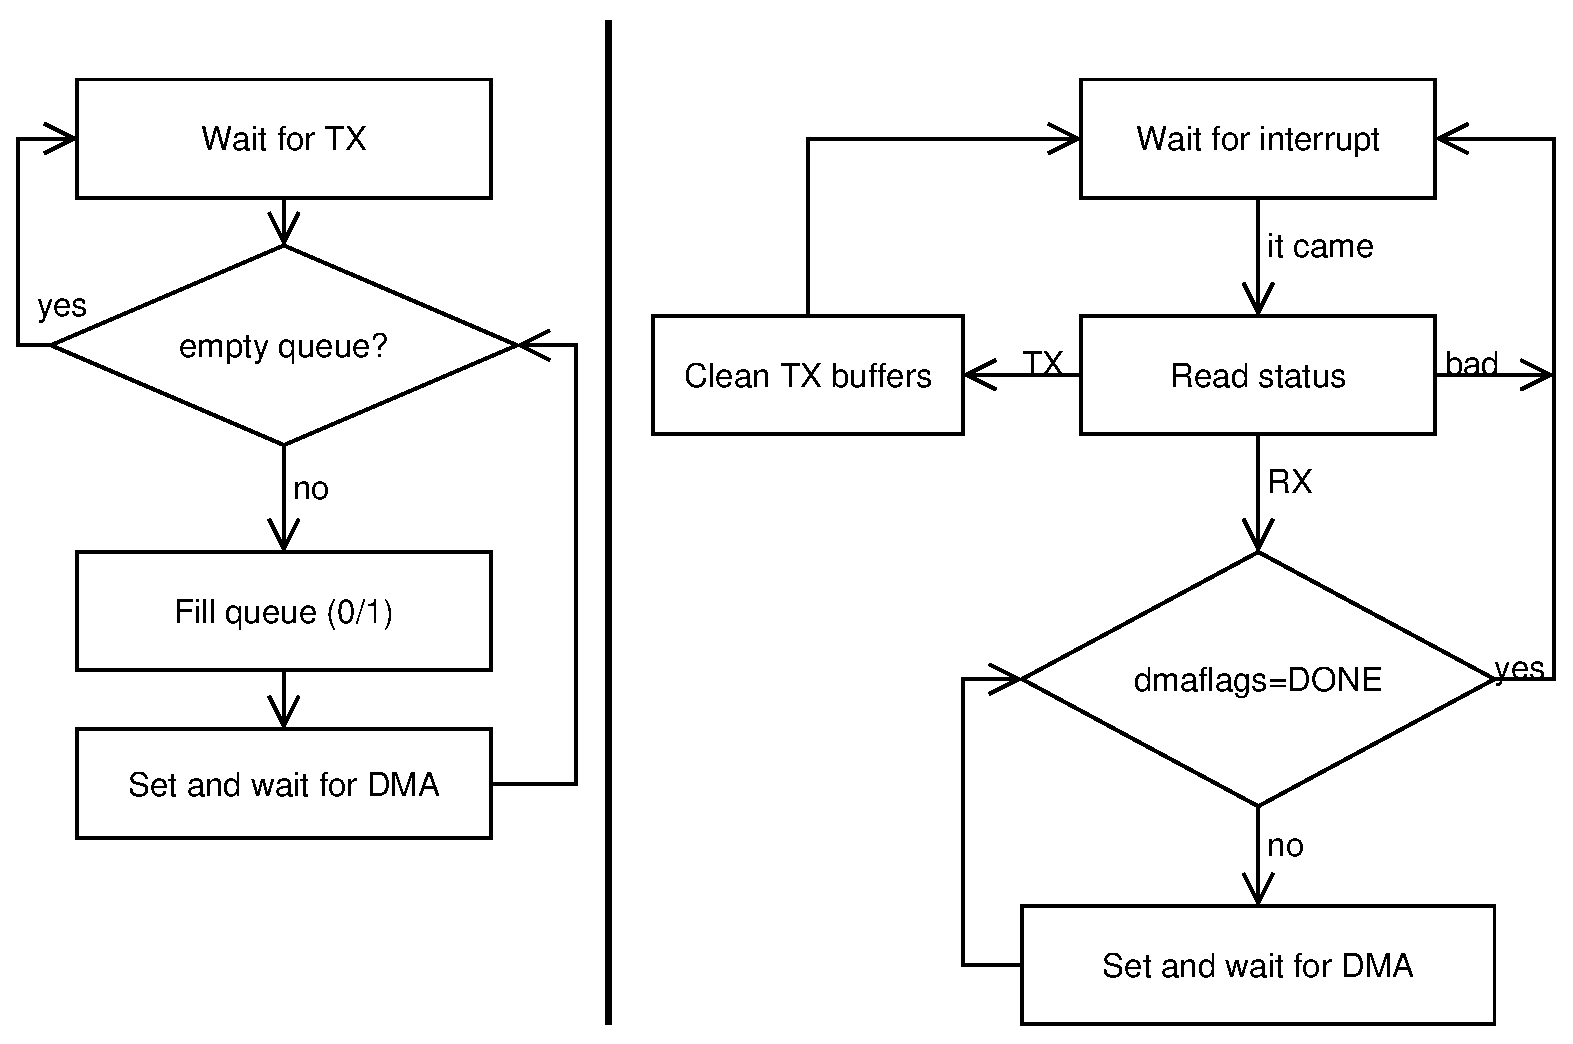
\includegraphics[width=10cm]{c6pcr}
      \caption{Princip ovladače v~diagramu}
    \end{center}
  \end{figure} \\ \indent
  Jako poslední zbývá vytvořené soubory -- \emph{c6pcreth\_real.c} (soubor se
  samotným ovladačem, zde je celé naše dosud vyvinuté úsilí),
  \emph{c6pcreth\_lkm.c} (obsahuje volání námi vytvořeného makra na tvorbu
  modulů) a soubor systému \emph{make} -- \emph{Makefile} (informace o způsobu
  překladu).
